\documentclass[10pt,a4paper]{article}
%\usepackage[table]{xcolor}
%\usepackage{float}
\usepackage[spanish]{babel}
\usepackage{amsmath}
%\usepackage{amssymb}
\usepackage{graphicx}
%\usepackage{amsfonts}
\usepackage[utf8]{inputenx}
\usepackage{pdfpages}
\usepackage{listings}
%\usepackage{algorithm2e}
\usepackage{listings}
%\usepackage{pdfpages}
\usepackage{tabularx}
\usepackage{color}
\usepackage{anysize}
\usepackage{fancyhdr}
\usepackage{ulem}
\usepackage{hyperref}
%\usepackage{caption}
\usepackage[font=footnotesize]{caption}
\definecolor{deepblue}{RGB}{0,0,153}
\definecolor{deepred}{RGB}{153,0,0}
\definecolor{deepgreen}{RGB}{51,102,0}
\definecolor{deepyellow}{RGB}{204,204,0}
\marginsize{2cm}{2cm}{1cm}{1.5cm} % depende de anysize
%\renewcommand*{\thefootnote}{\Roman{footnote}}
%\usepackage{hyperref}
%\hypersetup{
%    colorlinks=true,
%    citecolor=black,
%    filecolor=black,
%    linkcolor=black,
%    urlcolor=black,
%    linktoc=all
%}

% Custom colors
\usepackage{color}
\definecolor{deepblue}{rgb}{0,0,0.5}
\definecolor{deepred}{rgb}{0.6,0,0}
\definecolor{deepgreen}{rgb}{0,0.5,0}
\definecolor{orange}{rgb}{1,0.5,0}
\definecolor{grey}{rgb}{0.3,0.3,0.3}
\newcommand\bashstyle{\lstset{
language=Bash,
basicstyle={\small\ttfamily},
aboveskip=3mm,
columns=flexible,
breaklines=true,
breakatwhitespace=true,
tabsize=3,
belowskip=3mm,
otherkeywords={self},             % Add keywords here
keywordstyle=\ttfamily\color{blue},
emph={MyClass,__init__},          % Custom highlighting
emphstyle=\ttfamily\color{deepred},    % Custom highlighting style
stringstyle=\color{deepgreen},
morekeywords={peter@kbpet},
alsoletter={:~\$},
morekeywords=[2]{peter@kbpet:},
keywordstyle=[2]{\color{red}},
literate=
         {:}{{\textcolor{red}{:}}}1
         {~}{{\textcolor{red}{\textasciitilde}}}1,
frame=tb,                         % Any extra options here
showstringspaces=false            % 
}}
\lstnewenvironment{bash}[1][]
{
\bashstyle
\lstset{#1}
}
{}

%\title{Multímetros en Corriente Continua}
\title{Universidad de Buenos Aires - FIUBA \\
		66.20 Organización de Computadoras \\
		Trabajo Práctico 1: Assembly Mips\\}
\author{	Joaquin Segui, \textit{Padrón Nro. 91.451}                     \\
            \texttt{ segui.joaquin@gmail.com }                                          \\[2.5ex]
            Pernin Alejandro, \textit{Padrón Nro. 92.216}                     \\
            \texttt{ale.pernin@gmail.com}                                              \\[2.5ex]
            Menniti Sebastián Ezequiel, \textit{Padrón Nro. 93.445}                     \\
            \texttt{ mennitise@gmail.com }                                              \\[2.5ex]}
\date{}

%\lfoot{asdasd}


\begin{document}
%\includepdf{attachments/caratula.pdf}


%\newpage\null\thispagestyle{empty}\newpage
\maketitle\thispagestyle{empty}

\newpage\null\thispagestyle{empty}%\newpage

%\newpage
%\tableofcontents

%\newpage\null\thispagestyle{empty}\newpage

\section{Introducción}

Se implementó un programa, en lenguaje C, que se encarga de multiplicar matrices de números reales, representados en punto flotante de doble precisión. A diferencia del trabajo anterior, la función encargada de la multiplicación de las matrices se encuentra escrita en el lenguaje Assembly Mips.


\section{Diseño e Implementación}

Dada las limitaciones del assembly Mips, fue necesario realizar algunos cambios respecto de la entrega anterior

\begin{itemize}
	\item Representar las matrices como un unico arreglo de doubles.
	\item Diseñar el manejo de los argumentos mediante el stack.
	\item Modificar el algoritmo de multiplicación para contemplar errores de MIPS\footnote{Ver sección \ref{sec:MIPS}}.
\end{itemize}

Para manejar diversas variables dentro del programa, se utilizo un Stack Frame de 32 bytes.

	\begin{center}
			{\footnotesize \begin{tabular}{ |l|c| }

			\hline
				52 & columnas 2 \\ \hline
				48 & columnas 1 \\ \hline	
				44 & a3 (filas 1) \\ \hline
				40 & a2 (double* src1) \\ \hline
				36 & a1 (double* src2) \\ \hline
				32 & a0 (double* dest) \\ \hline
				28 & ra \\ \hline
				24 & fp \\ \hline
				20 & gp \\ \hline
				16 & i \\ \hline
				12 & j \\ \hline
				8 & k \\ \hline
				4 & (not used) \\ \hline
				0 & accum \\ \hline
				
			\end{tabular}}\captionof{table}{Stack Frame}\label{tab:regtension}
	\end{center}

Alli se alojan los valores empleados para los controles de los ciclos y el acumulador auxiliar para la multiplicación. Si bien la posición 4 no se utiliza, el frame debe ser multiplo de 8 bytes y por ello se mantienen los 32 bytes.

\section{Comandos para compilar el programa}
	\subsection{Copiar a VM}
		Dado que el programa se corre dentro de la maquina virtual gxemul, se facilita un script en bash que copia el contenido de la carpeta en el guest (considerando la configuración default vista en clase). Para ello invocar desde el host
		\begin{bash}
		copiar_tp.sh
		\end{bash}
		 el mismo se copiará en \textit{/root/tp1}.

	\subsection{Compilacion y Ejecucion}
		Para facilitar la compilacion se utiliza un \textit{Makefile}, para invocar la compilación del programa ejecutar desde una consola, dentro del mismo directorio que el código fuente:
		\begin{bash}
		make
		\end{bash}

		Asimismo se proviciona un script que realiza pruebas con un set de datos preexistente, para invocarlo: 
		\begin{bash}
		bash pruebas_mips.sh
		\end{bash}

\section{Pruebas}
	En esta sección se detallarán las pruebas realizadas. Los archivos utilizados se encuentran el el directorio \textit{test\_files}.
	\subsection{Casos Exitosos}
		Los casos exitosos están comprendidos por los set de datos \textit{test1} y \	textit{test2}.	
		En el caso del	 primero:\	
	
		\lstinputlisting[basicstyle=\footnotesize]{../src/test_files/test1.txt}
	
		Representa la operación
		\begin{center}
		$\begin{pmatrix}
		1 & 2
		\end{pmatrix}
		*
		\begin{pmatrix}
		1 & 0 & 4 \\ 5 & 1 & 3
		\end{pmatrix}
		=
		\begin{pmatrix}
		11 & 2 & 10
		\end{pmatrix}
		$
		\end{center}
	
		cuya salida por consola mediante el script de pruebas es
	
		\begin{bash}
		1x3 11 2 10
		\end{bash}
	
		como es esperable.\\
	
		El segundo set de datos es:
		\lstinputlisting[basicstyle=\footnotesize]{../src/test_files/test2.txt}
	
		representando las operaciones
	
		\begin{center}
		$\begin{pmatrix}
		1 \\ 2 \\ 3
		\end{pmatrix}
		*
		\begin{pmatrix}
		0 & 3 & 1
		\end{pmatrix}
		=
		\begin{pmatrix}
		0 & 3 & 1 \\ 0 & 6 & 2 \\ 0 & 9 & 3
		\end{pmatrix}
		$\end{center}
	
		\begin{center}
		$\begin{pmatrix}
		1 & 3
		\end{pmatrix}
		*
		\begin{pmatrix}
		1 & 0 & 4 \\ 5 & 1 & 0
		\end{pmatrix}
		=
		\begin{pmatrix}
		16 & 3 & 4
		\end{pmatrix}
		$\end{center}
	
		cuya salida se obtuvo correctamente
		
		\begin{bash}
		3x3 2.22507e-308 3 1 3.33761e-308 6 2 4.45015e-308 9 3 
		1x3 16 3 4
		\end{bash}

	\subsection{Casos de error}
		Como casos de error del programa probamos matrices incompatibles para su multiplicacion y matrices mal definidas.

		Uno de estos casos es el de tener dos matrices cuyas dimensiones hacen incompatibles la multiplicación entre sí. Este es el caso del set \textit{test3}.

		\lstinputlisting[basicstyle=\footnotesize]{../src/test_files/test3.txt}
		\begin{center}
		$\begin{pmatrix}
		1 & 2
		\end{pmatrix}
		*
		\begin{pmatrix}
		1 & 0 & 4
		\end{pmatrix}
		$\end{center}

		Al ejecutar dicha prueba, el programa termina con el siguiente mensaje:

		\begin{bash}
		Dimensiones no compatibles para multiplicar
		\end{bash}

		Otra prueba es tener una cantidad impar de matrices, por lo cuál una no podrá ser multiplicada. Por ejemplo \textit{test4}.

		\lstinputlisting[basicstyle=\footnotesize]{../src/test_files/test4.txt}
		
		Como resultado arroja

		\begin{bash}
		3x3 2.22507e-308 3 1 3.33761e-308 6 2 4.45015e-308 9 3
		Fallo al leer dimensiones
		\end{bash}

		Otros casos de prueba, consisten en definir dimensiones de matrices inconsistentes con la cantidad de elementos leidos. Al ver \textit{test5}

		\lstinputlisting[basicstyle=\footnotesize]{../src/test_files/test5.txt}

		\begin{center}
		$\begin{pmatrix}
		1 \\ 2 \\ X
		\end{pmatrix}
		*
		\begin{pmatrix}
		0 & 3 & 1
		\end{pmatrix}
		$\end{center}

		si bien las dimensiones declaradas son compatibles para su multiplicación, los elementos provistos son inconsistentes. Dicha prueba arroja:

		\begin{bash}
		Cantidad elementos distinta a dimensiones de matriz
		\end{bash}

	\subsection{Comportamiento en MIPS}\label{sec:MIPS}
		En la anterior implementación de este algoritmo en MIPS, observamos que los resultados que debieran dar 0, dan números extremadamente chicos expresados en notación científica. Observando este comportamiento sólo en el \textit{guest} y no el \textit{host} lo que nos llevó a efectuar un posterior análisis. Por ejemplo el caso de prueba exitoso 2 (\textit{test2.txt}) arrojaba como primer resultado:
		\begin{bash}
		3x3 2.22507e-308 3 1 3.33761e-308 6 2 4.45015e-308 9 3
		\end{bash}

		Para rastrear el origen de dicho problema se hicieron diveros prints y luego se empleó una prueba unitaria para ejemplificar dicho inconveniente (\textit{comportamiento\_mips.c)}. 

		\begin{figure}[h]
			\centering
			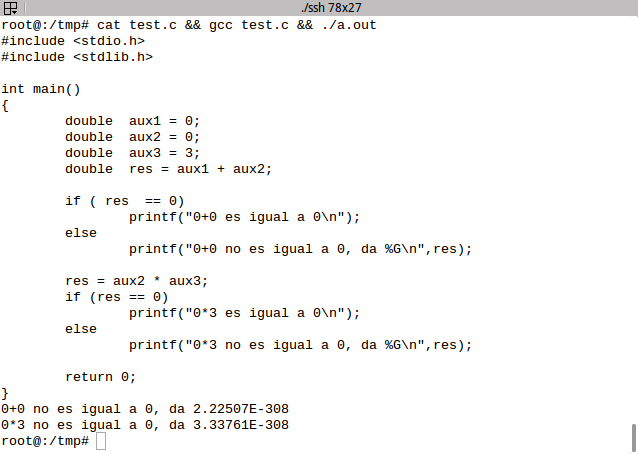
\includegraphics[scale=0.45]{images/raro.png}\caption{Prueba Comportamiento Mips}
		\end{figure}

		Como es observable, el problema radica en las operaciones de suma y multiplicación cuando uno de sus operandos es el cero. 

		Para evitar este comportamiento, el algoritmo compara si alguno de los elementos de las matrices a ser multiplicado es nulo. De serlo, el acumulador permanece igual y se continua en el siguiente ciclo. De esta manera el acumulador se mantiene inalterado por dicho comportamiento.

\section{Conclusiones}
	Mediante el estudio e implementación de algoritmos en assembly MIPS, pudimos observar cómo funciones sencillas en un lenguaje de alto nivel (desde este punto de vista) se traducen en múltiples instrucciones de bajo nivel en diversas ocasiones siendo éste mucho más complejo.

	Asimismo entendimos la importancia de establecer convenciones a la hora de realizar llamadas entre funciones para que dichas no sólo puedan realizarse pasajes de argumentos y resultados, sino para que durante el funcionamiento de una de ellas no afecte de manera indebida la otra.

	A lo largo del desarrollo de este TP, como guía observamos y estudiamos el código assembly obtenido mediante el compilador de diversos programas sencillos, resultando de gran utilidad.

\newpage
\section{Codigo fuente del programa}

\subsection{En lenguaje C}

\lstinputlisting[
			language=C,
			basicstyle=\footnotesize,
			numbers=left,
			stepnumber=1,
			numbersep=4pt,
			tabsize=2,
			otherkeywords={self}, 
			keywordstyle=\color{deepred},
			stringstyle=\color{deepgreen},
			commentstyle=\color{deepblue},
			]{../src/main.c}

\newpage
\subsection{Funcion en MIPS32}

\lstinputlisting[
			language=Assembler,
			basicstyle=\footnotesize,
			numbers=left,
			stepnumber=1,
			numbersep=4pt,
			tabsize=2,
			otherkeywords={self}, 
			keywordstyle=\color{deepred},
			stringstyle=\color{deepgreen},
			commentstyle=\color{deepblue},
			]{../src/myMultiplicar.S}

\newpage\thispagestyle{empty}
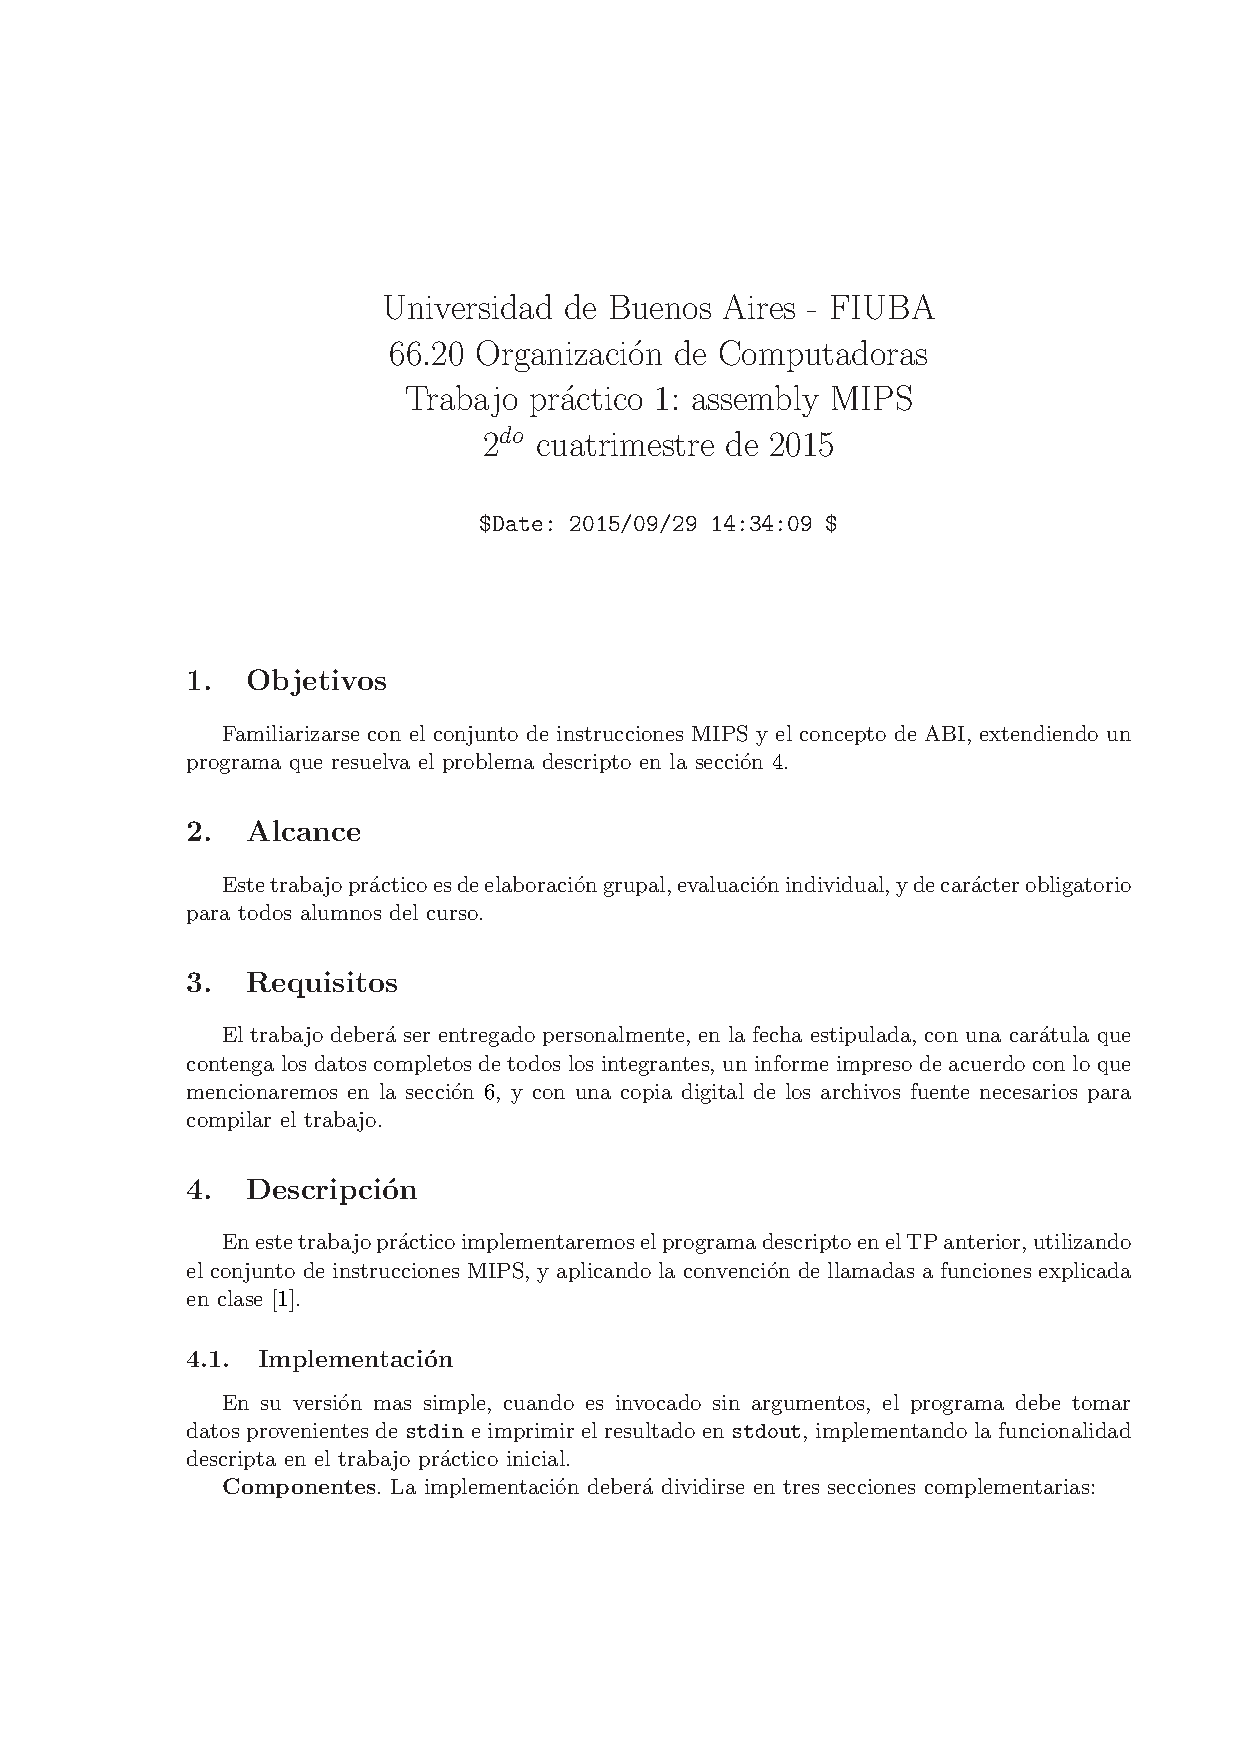
\includepdf[pages=1,pagecommand=\section{Enunciado}]{tp1-2015-2q.pdf}
\includepdf[pages=2-,]{tp1-2015-2q.pdf}

\end{document}